\documentclass[a4paper,11pt]{scrartcl}
\usepackage[utf8]{inputenc}
\usepackage{float}
\usepackage{amsmath}
\newtheorem{theorem}{Theorem}
\usepackage{graphicx}
\usepackage{caption}
\usepackage{subfig}
\usepackage{pdfpages}
\usepackage{wrapfig}
\usepackage{subfig}

%opening
\subject{Notes for Master's thesis\\
	Academic year 2022/2023s }
\title{Understanding the effect of opinions and behaviours on the spread of infectious diseases}
\subtitle{ }
\author{Riccardo Tessarin}
\date{ Email: riccardo.tessarin@studenti.unitn.it }



%% Stringhe per biblatex, compilare biber, pdflatex, biber pdflatex
\usepackage[english]{babel}
\usepackage[autostyle,italian=guillemets]{csquotes}                      
%% Per il corretto funzionamento di BibLatex
\usepackage[sorting=none,style=numeric-comp,backend=biber]{biblatex}
\addbibresource{bibliography.bib}

%pacchetto per i link cliccabili nel testo
\usepackage[hidelinks]{hyperref}
\hypersetup{ %impotazioni per i colori, in caso le volessi, a me non piacciono
	colorlinks=true,
	linkcolor=blue,
	filecolor=magenta,      
	urlcolor=cyan,
}

\urlstyle{same}


\begin{document}
	
	\maketitle
	\tableofcontents
	\pagebreak
	
	
\section{Multilayer Networks}

	\subsection{Epidemic spreading in multiplex networks influenced by opinion exchanges on vaccination}
	In the article \cite{AlvarezZuzek2017} it is described a 2 layers Network of Networks (NoN) system.
	Here the spread of the disease is described with a SIR mean field model, in which there is also the presence of a Vaccinate compartment, indicated with the letter V. 
	The opinion dynamics is based on the people belief on Vaccine. Simulating conversation with connected nodes, the opinion of people can change. When they totally trust in vaccine they get it and their probability of being infected decrease, according to a certain value $\omega$ that describe the efficiency of vaccine.
	"If two nodes have the same opinion orientation, one of them becomes more extremist with
	probability $p$, but if they have different opinion orientations one of the individuals becomes	more moderate with probability $q$". For simplicity, we consider $p + q = 1$. An important ratio can be defined and it is called $r$.
	\[r = p/q\] 
	$r$ is a parameter that define if the society is based more on compromise or dissuasion. These are two different mechanism. When $r<1$ the society is more moderate, although with $r>1$ the society tends to have more extremist opinions.
		
	\subsection{Choices, beliefs, and infectious disease dynamics }
	The work reported in \cite{AAuld2003} is interesting because  of the observations done on population behaviour. The main result obtained is that as a consequence of vaccine release there is an increasing in risky behaviour from the population. 
	The study is realized observing the spread of HIV virus, here the release of information about a future vaccine can cause a change in behaviour of forward looking agents. In the time before vaccine becomes available there is a lower infection rate, while when people becomes vaccinated they returns to their original habits. 
	The evolution of disease is described with a simple SI model. The population is described with 3 main indices: ages, preference types and infection status. A probability index of being infected is used. The higher is the numbers of contact, the higher is the $p_{ka}$ of being infected. \\
	Also a pessimistic view on the future development of disease cause more risky behaviour.
	Economic epidemiologies use instruments like microeconomic and econometrics to study and model choices during an epidemic. 
	
	\subsection{Evolutionary game theory and social learning can determine how vaccine scares unfold}
	In the article \cite{Bauch2012} it is presented the main mechanism for which vaccine scares people. The "free-rider problem" is a theory for which the vaccine-generated immunity is so great, that the risk related to the vaccine seems large, causing some individual to refuse the administrations of vaccine.
	The Game Theory is used to study how the choice of individuals influence and are influenced by the choices of others individuals. 
	In the paper is investigated the feedback loop connecting disease incidence and vaccinating behaviours. 
	\begin{itemize}
	\item  Disease incidence influence vaccinating behaviours;
	\item Vaccinating behaviour in turn influence disease incidence through herd immunity. 
	\end{itemize}
	The crucial assumption is
	
	In stage one, we formulated a social learning process based on the imitation dynamic of evolutionary game theory [18]. An individual samples others in the population at a constant rate. If the sampled person is playing a different strategy and is receiving a higher payoff, the individual switches to that strategy with a probability proportional to the expected gain in payoff.
	
	
	\subsection{A Mean-Field Analysis of a Network Behavioral–Epidemic Model}
	
	Articolo che mi ha mandato la professoressa \cite{Frieswijk2022}. Fanno una interessante analisi di un modello SIS + un modello comportamentale basato su Game Theory che mette assieme la fatica di usare le precauzioni, il costo economico di questo e le compara invece alla paura che lo spreading dell'infezione ha sull'incentivare le persone ha seguire le indicazioni.
	There are two interesting pay off function, that rule with a Poisson clock the rates at which behaviour of people change. 
	The behaviour has here a very strong importance, because if an individual uses the self-protection its is sure to not contract the disease. 
	The letters has also a mean filed analysis of the model, to simplify its study and identify the relation between parameters. It is reported an example, with some calculated coefficients for the parameters and a Stability analysis of the solutions found are realized. 
	\\
	\textbf{Vedi note per i calcoli!} 
	
	
	\subsection{Misinformation can prevent the suppression of epidemics}
	In this article \cite{Sontag2022} it is presented a double layer model. The aim of the study is to show the relationship between a SIR model and an opinion dynamics model in which the effects of NPIs are considered.
	The opinion of each individual influence its action: they choose to use self protective measure and in this model the possibility of became Infectious is zero in this case. The population is here divided in 2 main categories Trusting and Distrusting (T and D). The opinion model here is interesting because there is quite a bit complex development for the opinion, based on the influence that have a better quality of information on others and also considering a "fading effect" that is the degradation of information when they are exchanged between people. 
	\\
	\textbf{Vedi note per i calcoli!}
	
	\subsection{The timing and nature of behavioural responses affect the course of epidemic}
	This is the most important article in this moment for my thesis \cite{Tyson_2020}.  The particularity of this work is on the opinion dynamics modelled created. Here there is not a vaccine to protect the population, that can avoid to become infected only with NPIs counter measures. The whole population is divided in 4 main group, for the level of protection they decide to adopt. The more one individual is cautious, the less are the probability of being infected.  
	The opinion evolution is simulated using contact with neighbours and conversations. Through this vehicle opinions can be influenced and a person can change its behaviour. 
	An amplification effect is also added to the model, to simulate the confirmation bias. Its main effect is to increase the size of peaks during the epidemic. 
	In the last part of the work a sensibility analysis is performed, testing the model at different parameter value and observing the evolution of a fast or slow epidemic. 
	
	\subsection{Triple contagion: a two-fears epidemic model}
	The article \cite{Epstein2021} is about a model that takes into account the effect of spread of 2 different fears: disease fear and vaccine fear. 
	The prevalence of one of this two fear cause a specific dynamics in epidemics evolution. 
	When the number of infected individuals in a standard SIR model increase, the disease fear cause people to adopt self protective measure and to vaccine. 
	This behaviour is analysed, and the result are very interesting, in particular the results obtained in the sensitivity analysis can be very useful to model response to vaccine, scare of vaccine side effects. The final model is visible in \ref{fig:three_fear}.
	
	\begin{figure}[H]
		\centering
		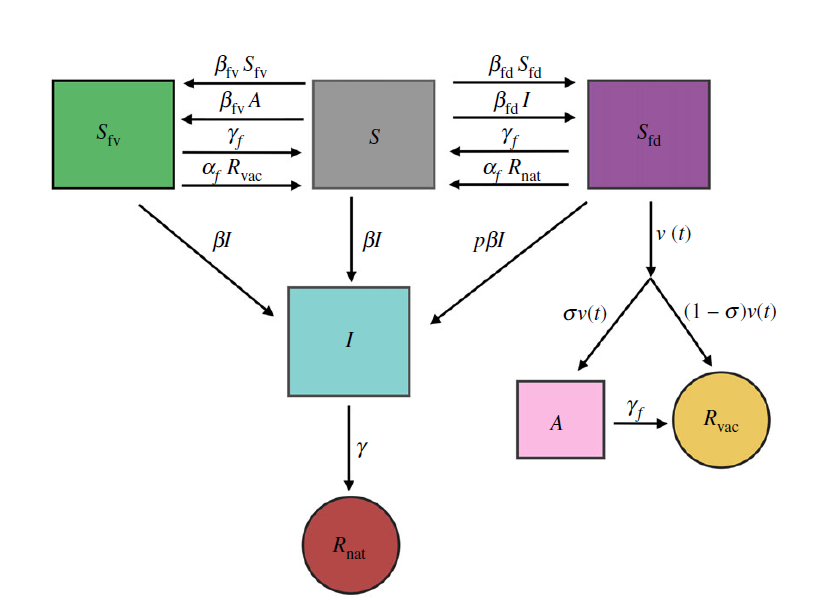
\includegraphics[width=0.7\textwidth]{images_note/three_fears.png}
		\caption{Mena field model explained in \cite{Epstein2021}. It a modified SIR model, very interesting! } 
		\label{fig:three_fear}
	\end{figure}
	
	
		\subsection{Optimal shutdown strategies}
		In the article \cite{Barlow2021}, a two layer model is presented for study the evolution of COVID-19 between March 2020 to September 2020 and the economic costs. 
		Lockdown is an important measure for saving human life against aggressive disease and slow down the evolution of pandemic. However, there is an important economic cost caused by this measure. 
		In this work is analysed the beneficial effects of lock down and its drawbacks and is presented an optimal control problem used to find the best modality for its use. 
		
		
		
		An interesting compartmental model for  describe the economic cost related to the disease is implemented. There is a $Q$ compartment composed by 5 subset, used to described different quarantine regimes. 
		

	
	\subsection{Multi-layer network approach in modelling epidemics in an urban town}
	\textbf{Very interesting work!} The article \cite{Turker2021}  present a  model for describe a town in a very detailed way. The purpose is to create a multi-layer structure in which individuals are nodes linked to others considering their family (house level), their work or school, and which type of work they do. There is a differentiation between essential workers that must go physically to work, and others that can work remotely. 
	
	The resulting network is composed by 7 layers and it is used to calculate different levels of lockdowns. The main result is that the 2 layers that contribute more to spreading the contagion are School and Friendship.
	In particular the friendship level is the one for which the lowest $\beta$ value is sufficent to generate an epidemic. 
	
	In the article there is also a very complete presentation of the state of the art in multi layer networks, visible in the following figure, to remember all the citations present, look at figure \ref{fig:fonti}.
	
	\begin{figure}[H]
		\centering
		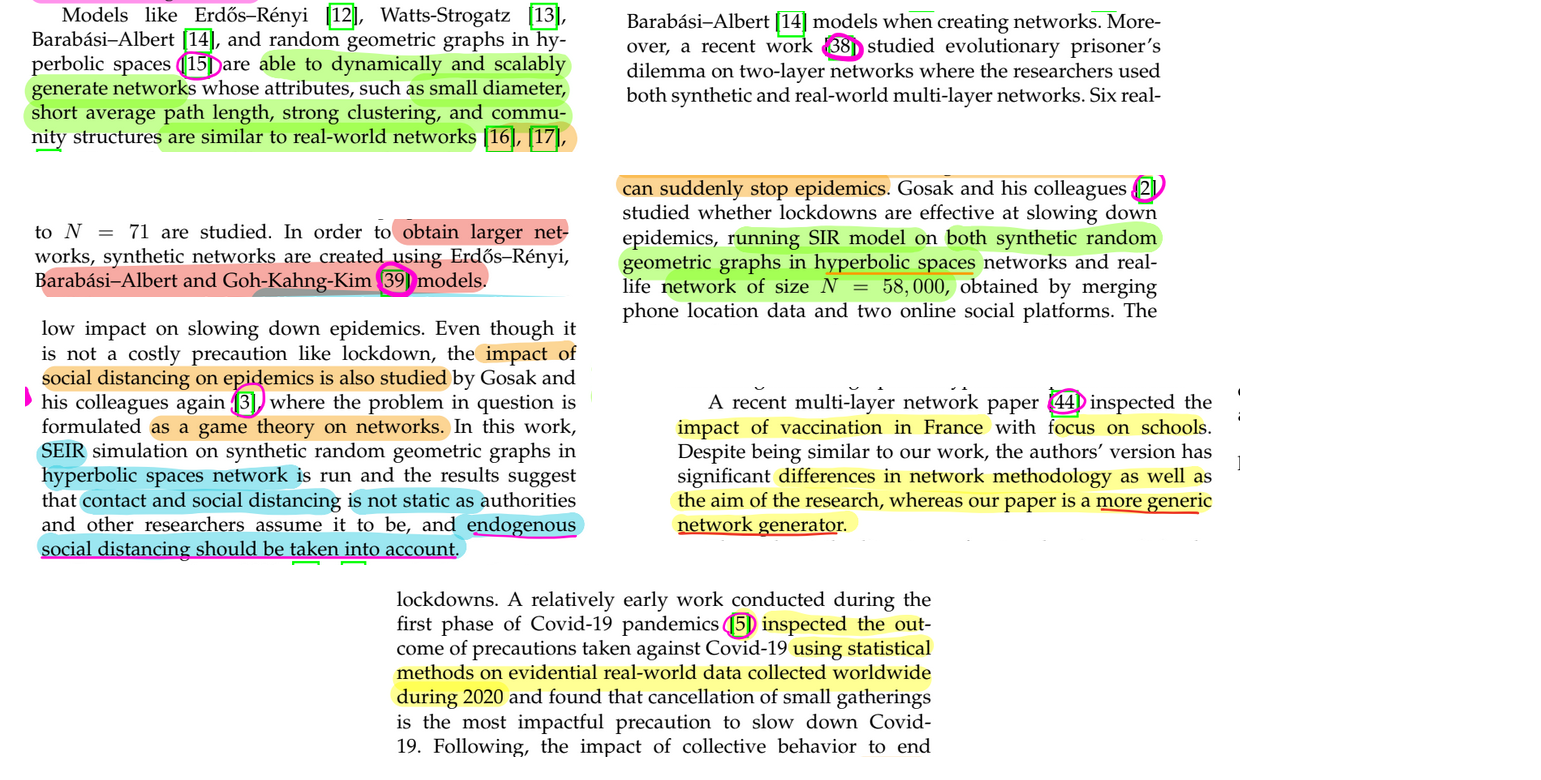
\includegraphics[width=0.9\textwidth]{images_note/fonti_da_articolo.png}
		\caption{Fonti molto interessanti da tenere bene a mente! } 
		\label{fig:fonti}
	\end{figure}
	
	
	
\section{Network modelling}  	
A possible way to describe and realize a giant network of  interconnection between individuals is using the algorithm presented in \cite{Molloy1995}. The Molloy-Reed algorithm establish a criterium for a network to be of the Giant type. \textbf{This topic must be understood well!}

\subsection{Emergence of Soft Communities from Geometric Preferential Attachment }
In this article \cite{Zuev2015}it is presented the mathematical method developed for realize a graph that is similar in structure to Real Networks.
The method consist in GPA (geometric preferential attachment) that is implemented in an hyperbolic description of the space. Two forces drive the formation of graph structure during its evolution (the increase of node number and links): popularity and similarity.
Popularity is the property of a node to attract connection if it has an high degree number. Similarity is the formation of link between nodes that are similar under some defined characteristic. 

\textbf{Look at notes for article detailed summary, and consider the math methods section for implementation in your network!}

\section{Opinion dynamic}

	\subsection{A framework to analyze opinion formation models}
	In \cite{Devia2022} the focus of research is to analyse the behaviour of different method implemented to predict the evolution of opinion, and verify their consistency with real data. The main result of the work is the demonstration that often the predicting methods used have a tendency over consensus of opinion. Instead, real opinion can change in very different ways. 
	  	
	  Opinion model must include mechanism to produce dissensus, clustering or polarization. These can be realized using stochastic and random effects. Real evolution of opinion lead to transient state, not consensus. Initial opinion has a strong effect on final distribution: assume a random distribution for this initial condition can influence deeply the model performance. 
	  
	  Interesting model analysed: Bounded Confidence, Weighted median and Quantum Game
	  
	  \textbf{Guarda come funziona Freidrick-Johnson model che sembra interessante!!}
	  
	  \subsection{Social influence networks and opinion change}
	  In the article \cite{Friedkin99} it is analysed the process of interpersonal influence. 
	  
	  \subsection{Competing spreading processes on multiplex networks: awareness and epidemics}
	  Epidemic-like spreading processes on top of multilayered interconnected complex networks reveal a rich phase diagram of intertwined competition effects. A recent study by the authors [Granell et al. Phys. Rev. Lett. 111, 128701 (2013)] presented the analysis of the interrelation between two processes accounting for
	  the spreading of an epidemics, and the spreading of information awareness to prevent its infection, on top of multiplex networks. The results in the case in which awareness implies total immunization to the disease, revealed the existence of a metacritical point at which the critical onset of the epidemics starts depending on the reaching of the awareness process. Here we present a full analysis of these critical properties in the more general scenario where the awareness spreading does not imply total immunization, and where infection does
	  not imply immediate awareness of it. We find the critical relation between both competing processes for a wide spectrum of parameters representing the interaction between them. We also analyze the consequences of a massive broadcast of awareness (mass media) on the final outcome of the epidemic incidence. Importantly enough, the mass media makes the metacritical point to disappear. The results reveal that the main finding i.e. existence of a metacritical point, is rooted on the competition principle and holds for a large set of scenarios.
	  	
	  	
\section{Other articles}
	
		\subsection{Effect of hand hygiene}
		In \cite{Aiello2008} there is the description of an important research developed to verify the impact of hand hygiene on the infection disease risk. There is no information useful for a network model, but it is assessed the efficiency of prophylactic behaviours in preventing gastrointestinal and respiratory infections. 
		
		
\section{Reviews}

\subsection{A review and agenda for integrated disease models including social and behavioural factors}
Social and behavioural factors are critical to the emergence, spread and containment of human disease, and are key determinants of the course, duration and outcomes of disease outbreaks. Recent epidemics of Ebola in West Africa and coronavirus disease 2019 (COVID-19) globally have reinforced the importance of developing infectious disease models that better integrate social and behavioural dynamics and theories. Meanwhile, the growth in capacity, coordination and prioritization of social science research and of risk communication and community engagement (RCCE) practice within the
current pandemic response provides an opportunity for collaboration among epidemiological modellers, social scientists and RCCE practitioners towards a mutually beneficial research and practice agenda. Here, we provide a review of the current modelling methodologies and describe the challenges and opportunities for integrating them with social science research and RCCE practice. Finally, we set out an agenda for advancing transdisciplinary collaboration for integrated disease modelling and for more robust policy and practice for reducing disease transmission.	
	
	  	
\printbibliography[heading=bibintoc, title={Bibliography}]



\end{document}
